\subsection{Oscilloscope}
An oscilloscope is a popular lab tool used to output voltage as a function of time.
Modern oscilloscopes often use \gls{lcd} displays and rasterize output. 
However, some older models include a \gls{crt} vector display.

To draw on such an oscilloscope, the device must support at least two input channels, and the ability to draw in X-Y mode.
In this mode, two of the input channels (usually Ch1 and Ch2) governs the electron ray deflectors, which are controlled through electrostatics. 
This is different from the normal mode where the beam moves to the right with a constant speed \( t \) and one of the channels determine the amplitude.

The voltage on channel one will normally decide the beam's horizontal X position, and channel two its vertical Y position.
If the channels are provided a constant voltage, a dot will be displayed on the screen - in contrast to normal mode, where a line would be drawn.
To draw a line on the oscilloscope in X-Y mode, frequent changes to the voltage of one or both channels is necessary to make the image remain on the screen. //TODO Lima: For our osc this is true, but other types may be different
Alternating the voltage on one channel only, will produce a horizontal or vertical line.

\subsubsection{Tektronix 2230}
The Tektronix 2230 oscilloscope, shown in figure \ref{fig:oscilloscope}, has been used in this project to display the vectorized output.
The device has two input channels and supports an input frequency up to 100 MHz, where the voltage can range from 5mV to 5V per division.
A small \gls{crt} vector display is located on the front panel.
More detailed information can be found in the included manual\cite{tektronix2230}.

\begin{figure}[h!]
	\centering
	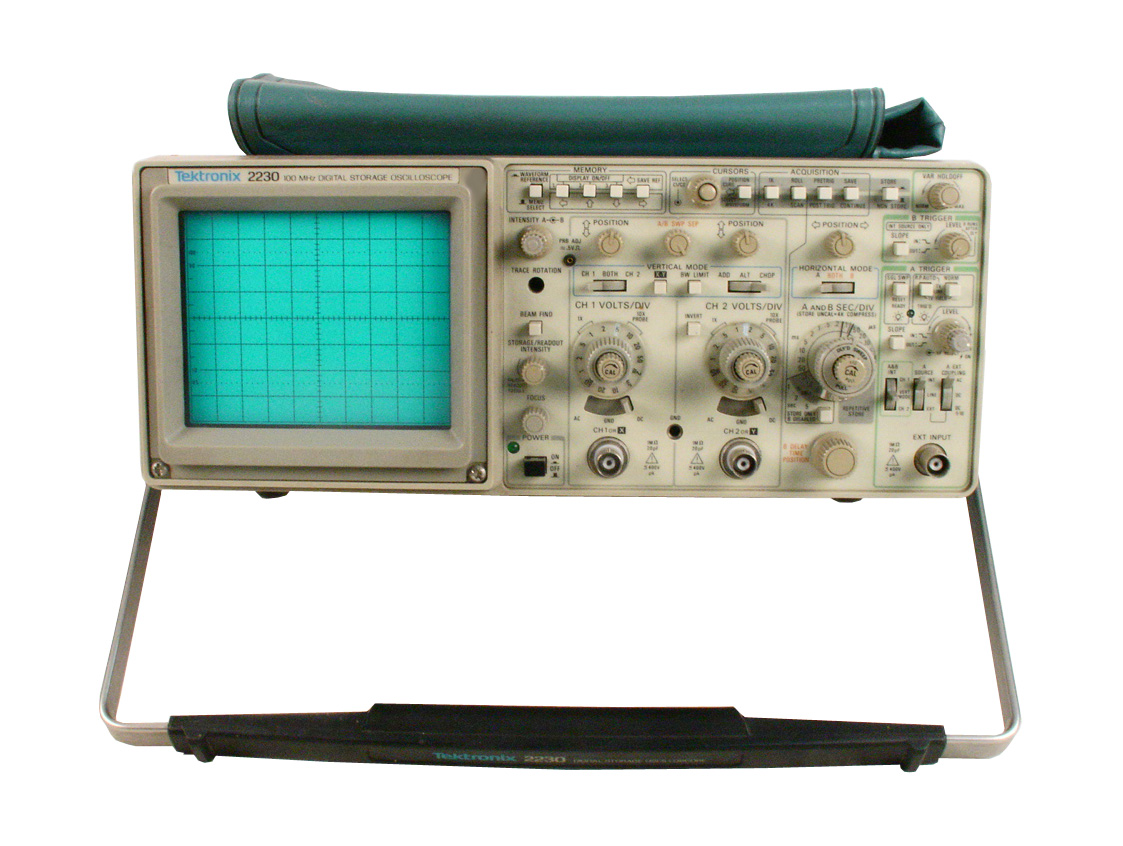
\includegraphics[width=0.6\linewidth]{images/oscilloscope.jpg}
    \caption{The Tektronix 2230}
    \label{fig:oscilloscope}
\end{figure}


